\documentclass[letterpaper, reqno,11pt]{article}
\usepackage[margin=1.0in]{geometry}
\usepackage{color,latexsym,amsmath,amssymb, listings}
\usepackage{color,latexsym,amsmath,amssymb,graphicx, float}

\newcommand{\RR}{\mathbb{R}}
\newcommand{\CC}{\mathbb{C}}
\newcommand{\ZZ}{\mathbb{Z}}
\newcommand{\QQ}{\mathbb{Q}}
\newcommand{\NN}{\mathbb{N}}
\newcommand{\st}{\mathrm{ s.t.}\ }

\begin{document}
\pagenumbering{arabic}
\title{Phys 301 Tutorial 2}
\date{September 22, 2021}
\author{Xander Naumenko\\
Nathan Van Rumpt\\
Renu Rajamagesh\\
Sabrina Ashik
}
\newtheorem{thm}{Theorem}
\maketitle

\noindent {\bf 1.} The expression $\rho(x, y, z)=c\cdot \delta(x-3)$ represents a plane of charge passing through the point $(3, 0, 0)$ and parallel to the $yz$ plane. Since it has to represent a charge density and $\delta$ is in units of $m^{-1}$, $c$ must have units of $C/m^2$.  

For the sketch see figure \ref{fig:plane}. 

\begin{figure}[htbp]
\centering
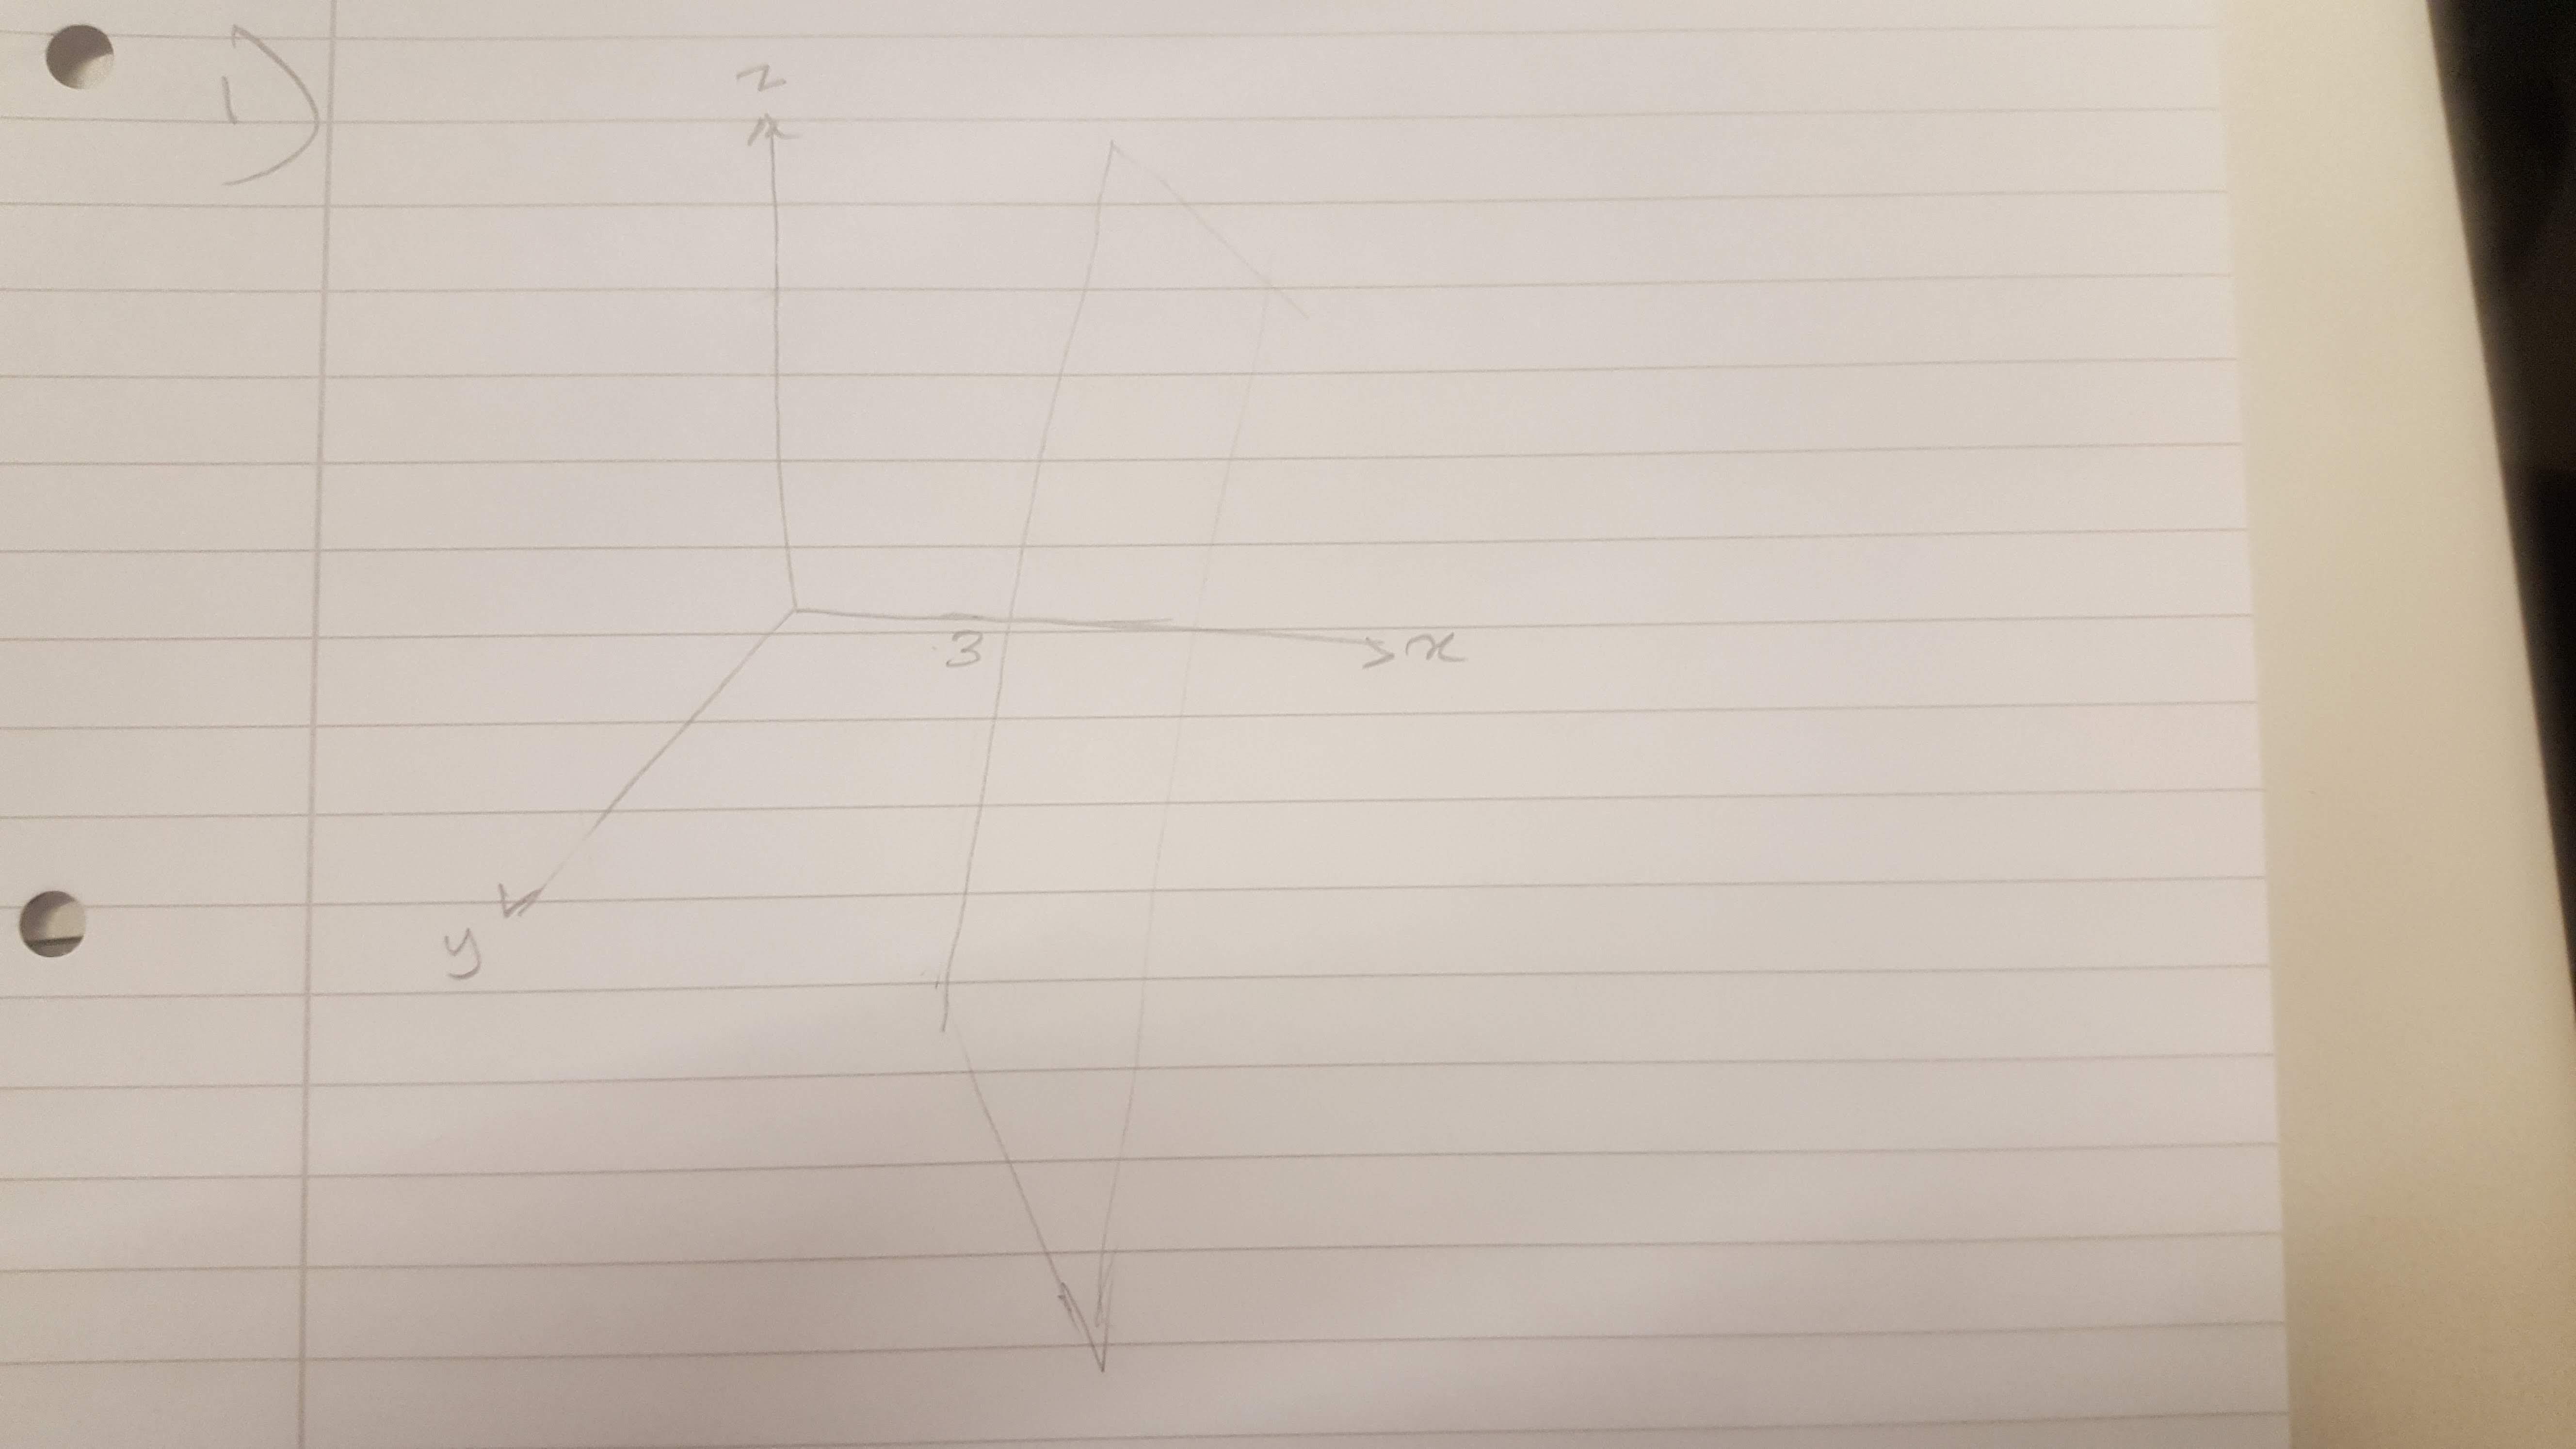
\includegraphics[width=\textwidth]{images/plane.jpg}
\caption{The plane represented by the function given in question 1. }
\label{fig:plane}
\end{figure}

\noindent {\bf 2a.} See figure \ref{fig:cylinder}. We chose cylindrical coordinates to solve the problem in. 

\begin{figure}[htbp]
\centering
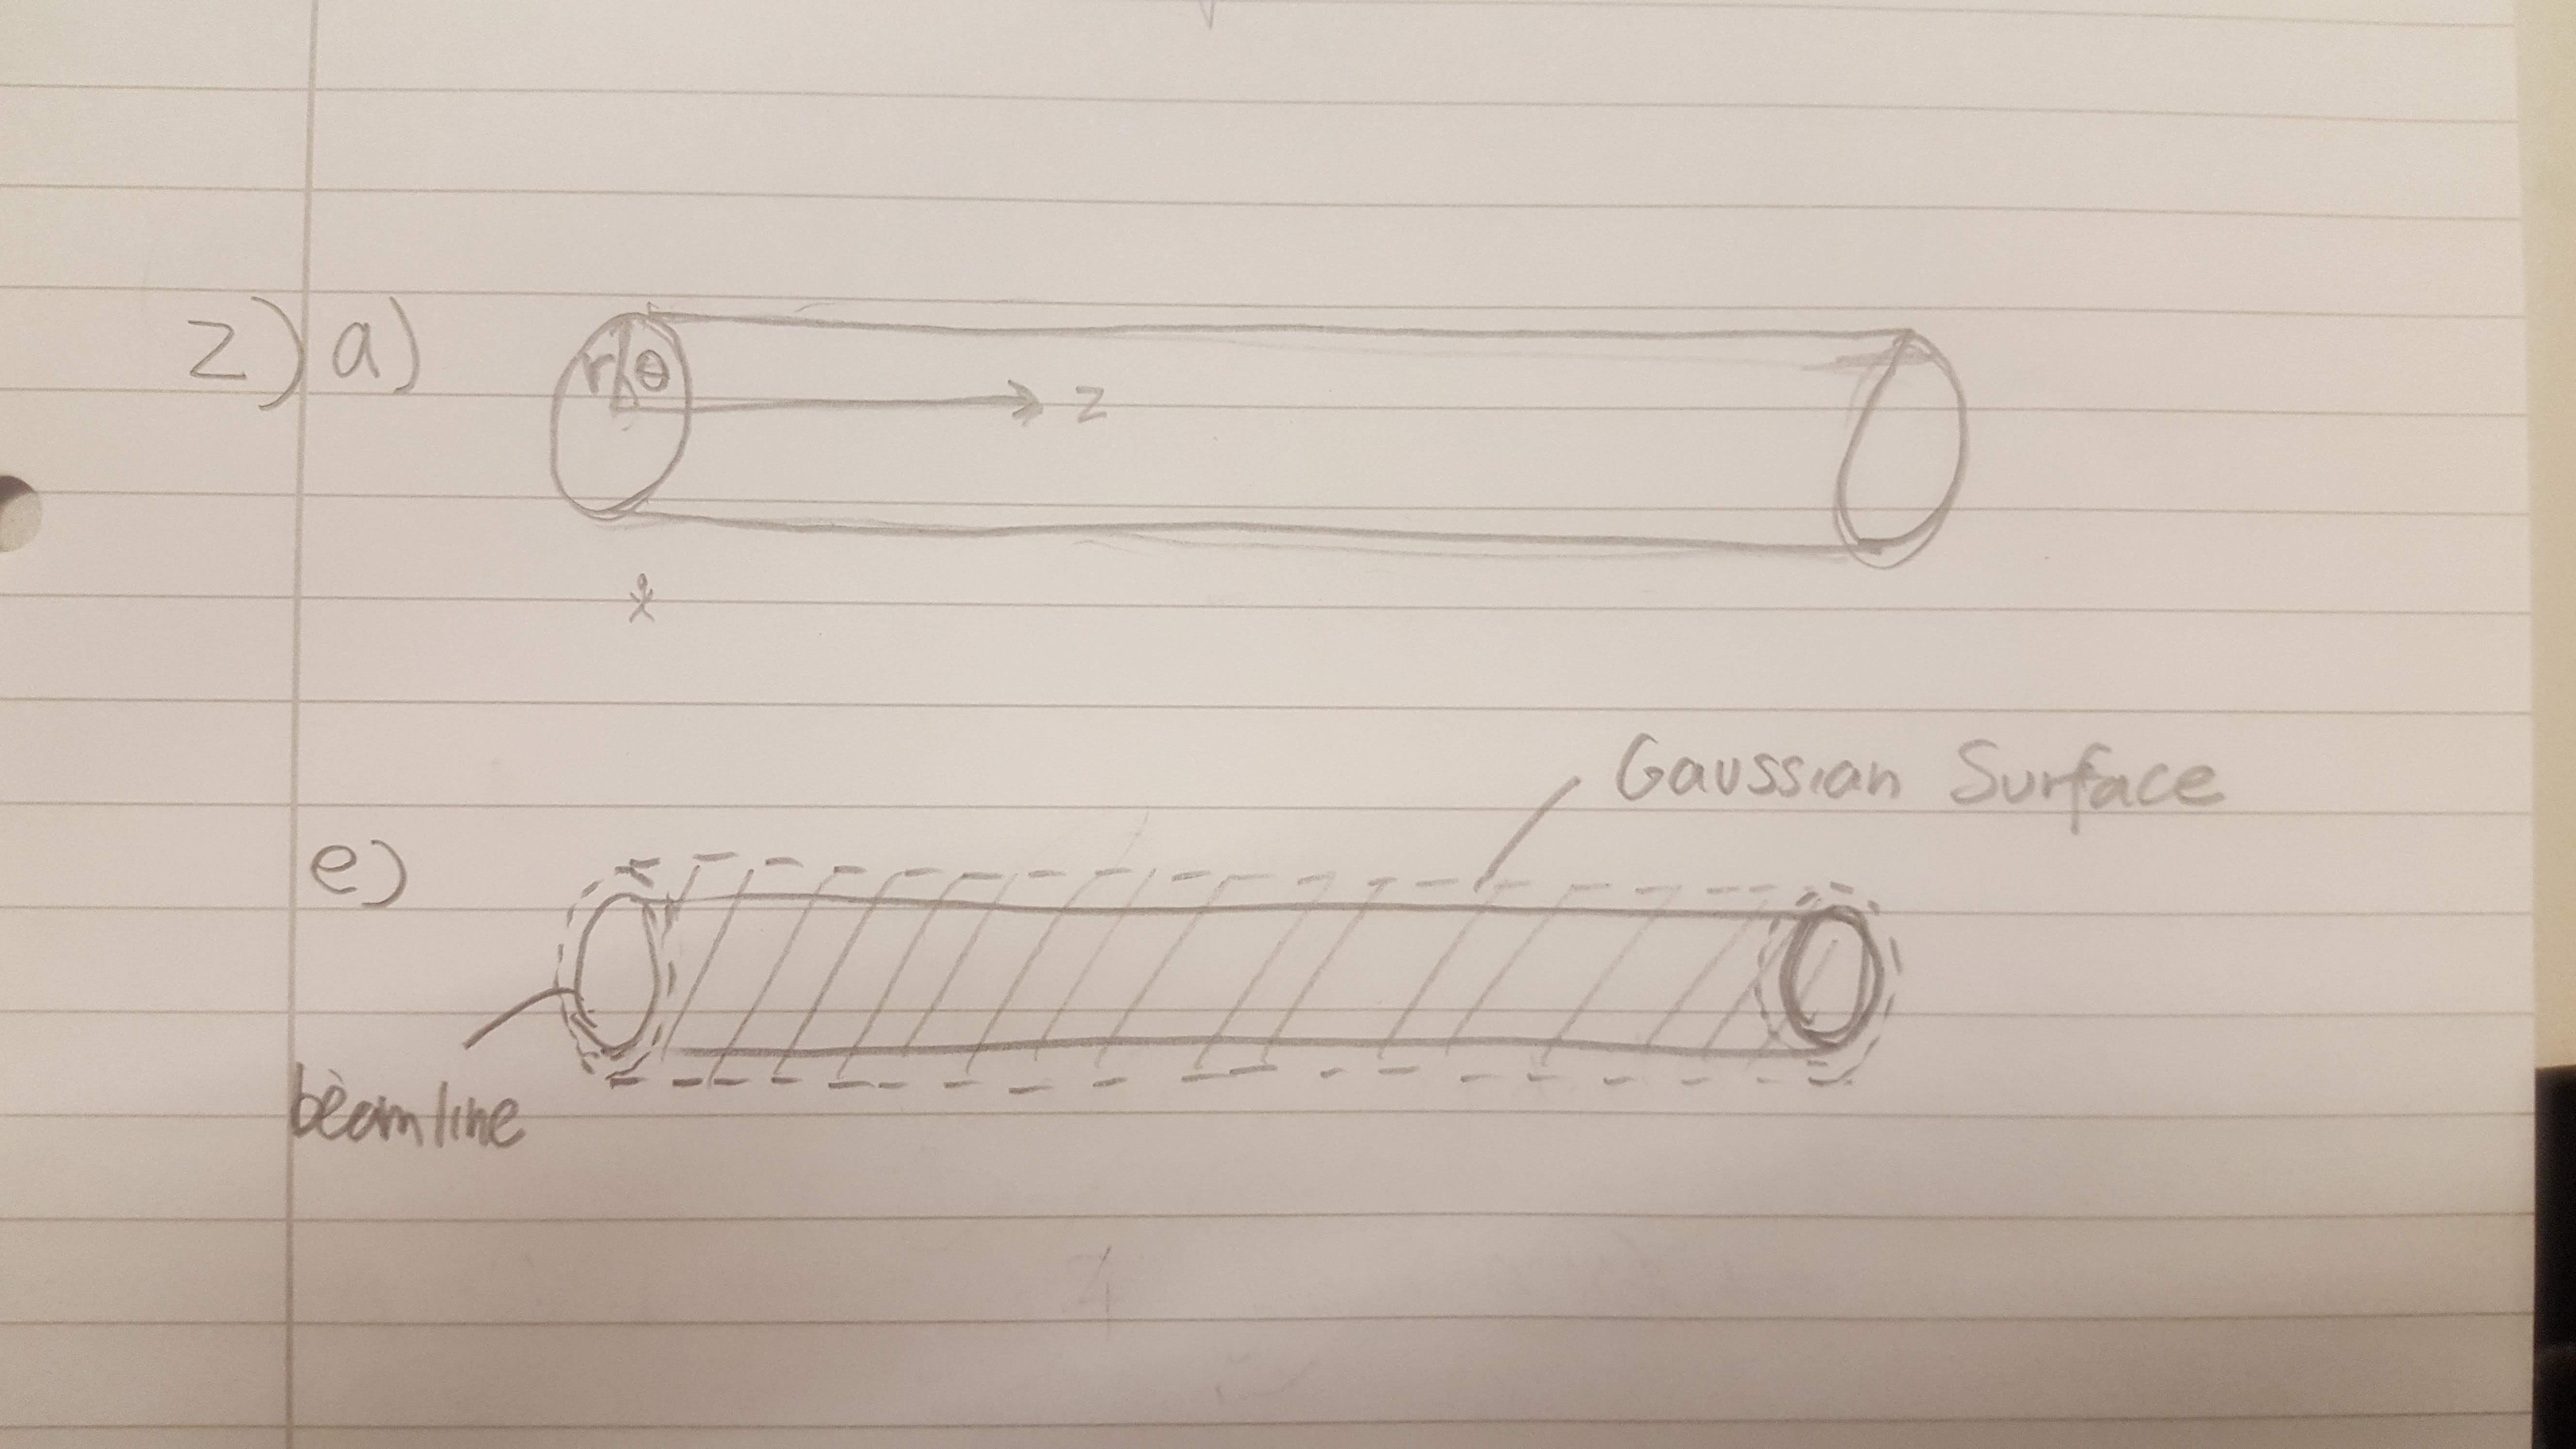
\includegraphics[width=\textwidth]{images/cylinder.jpg}
\caption{The cylinder represented in question 2a, along with our choice of the Gaussian surface for part e. }
\label{fig:cylinder}
\end{figure}

\noindent {\bf 2b.} We use cylindrical coordinates. Then the charge density will be 

$$
    \rho(r, \phi, z)=\delta(r-0.06)\sigma
$$

\noindent {\bf 2c.} Setting up the integral we get 

$$
    \int_0^{2\textnormal{ miles}}\int_0^{2\pi}\int_0^{0.06}\delta(r-0.06)\sigma r dr d\phi dz
$$
$$
    =2\pi\int_0^{2\textnormal{ miles}}0.06\sigma dz
$$

$$
    =0.12\pi\sigma 1609\cdot 2=386\pi\sigma\ C
$$

The units are correct, since the argument inside the integral has units of $C/m^2$, and we are integrating over two variables in units of meters ($z$ and $r$). 

\noindent {\bf 2d.} The electric field inside the pipe will be zero, because the pipe is presumably made out of a conductor and the electric field inside of a shell made out of a conductor is 0 (this would also be true in the case of an insulator, but would rely on a Gaussian surface inside it). For the outside, the electric field will point radially inward. Because of the symmetry of the geometry it must be going in a radial direction, and it goes inward because lightning carries a negative charge. 

\noindent {\bf 2e.} We will use a cylinder of length $l$ around the infinite cylinder to apply Gauss's law. This surface can be seen in figure \ref{fig:cylinder}. 

\noindent {\bf 2f.} The flux through either end of the cylinder will be zero since it is parallel to the radial direction. For the outer surface of the cylinder, using Gauss's law the flux will be

$$
    \Phi_E=EA=\frac{Q_{enc}}{\epsilon_0}
$$

\noindent {\bf 2g.} Because we are in cylindrical coordinates, we have 
$$
    d\vec A=rd\phi dz
$$

$d\vec A$ points radially outward. 

\noindent {\bf 2h.} Evaluating the integral: 

$$
    \iint \vec E\cdot d\vec A = \int_0^{2\pi}\int_0^{l} Erd\phi dz
$$

$$
    =2\pi E\cdot lr
$$

To find what $Q_{enclosed}$, we know the surface area is $2\pi r l$ and we know the surface charge density so computing we get 

$$
    \Phi_E=2\pi lrE = \frac{Q_{enc}}{\epsilon_0}=\frac{\sigma 2\pi 0.06 l}{\epsilon_0}
$$

$$
    \Rightarrow E=\frac{\sigma 0.06}{\epsilon_0 r}
$$

In vector notation, we have 

$$
    \vec E=\frac{-\sigma 0.06}{\epsilon_0 r} \hat r
$$

This is true only for $r>0.06$, inside the pipe the field is 0. 

\noindent {\bf 2i.} It does not affect the particles inside since the field is 0 inside, but it could affect the electronic equipment because there is a nonzero field produced around the field. 

{\noindent\bf Question 2j.} Let $V=0$ at $r=0$. Because the electric field is zero inside the cylinder, the potential at $r=0.06$ is also zero. For a general distance $d$ away, the potential would be 

$$
    V(d)=-\int_{0.06}^d\frac{-\sigma 0.06}{\epsilon_0 r}\hat r \cdot \hat r dr=\frac{0.06\sigma}{\epsilon_0}\log(r)\bigg|_{0.06}^d=\frac{0.06\sigma}{\epsilon_0}\log\frac{d}{0.06}
$$

This is valid for any $d>0.06$, for $d<=0.06$ then $V=0$. 

{\noindent\bf Question 2k.} By Gauss's law in its differential form, we know that 

$$
    \nabla \cdot \vec E=\frac{\rho}{\epsilon_0}
$$

Applying this, because the only charge is assumed to be on the wall of the pipe, the divergence of anywhere except the walls of the pipe must be zero. More specifically, plugging in our expression for $\rho$ found in part b, the divergence at all points in space is defined as 

$$
    \nabla\cdot\vec E=\frac{\sigma\delta(r-0.06)}{\epsilon_0}
$$

Thus the divergence is nonzero at all points such that $r=0.06$ and zero elsewhere. 


\end{document}